\section{Liturgy and the Logos}

\begin{wrapfigure}{rt}{.3\textwidth}
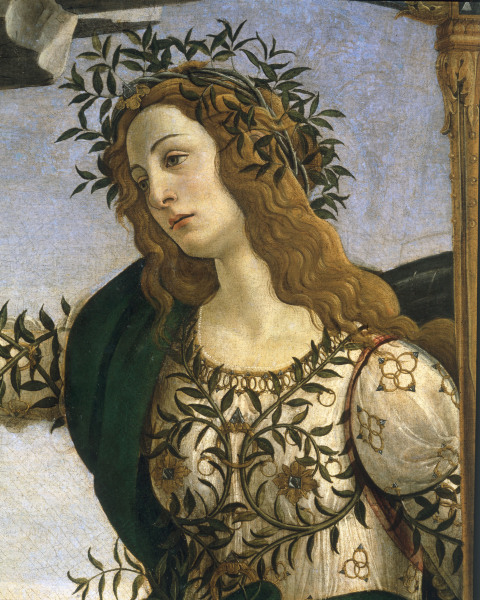
\includegraphics[width=.3\textwidth]{MInerva+botticelli.jpg}
\end{wrapfigure}

A popular refrain I hear from fellow Protestants is that ``meaningless rituals'', gestures, ``smells and bells'', or vain repetitions (a Scriptural phrase) won't help find favor with God. While I am certain that ritual can (and does) degenerate into ``those of darkness'' who are fascinated with the dead (Rene Guenon) and their debased conclaves or practices, the pre-existent Logos of the universe that created the world through its pattern entails that relationships between and among ``things'' exist, even at the lowest level. Anyway, if vain repetitions include all things which repeat themselves, then why do we always prefer beautiful pictures or soothing colors for certain environments, as opposed to the opposite? As Millinerd\footnote{\url{http://www.millinerd.com/2006/07/cultural-christianity.html}} pointed out, what happens when you ``lose the Faith'' in a church that used to be a drive-through? Will you be reminded by the stained glass on the wall? The spires? The ringing old church bell? Or the grease stains under the carpet? ``Cultural Christianity'' is the nave or ante-chamber of the Church -- the paintings on the walls of these early Churches were the Greek Philosophers like Heraclitus. It is Justin the Martyr, not Hippolytus, who should guide our thinking here.

The absolute consensus among anyone interested in Tradition is that some patterns are more significant (or more elevated) than others. Some Ideas are more fruitful than others. Some people are better than others, at least in the sense (and no one can disagree with this) that they are truer to their real Self. But what happens when you forget there is a higher Self that is more real? You turn to Revolution. And you hate your patrimony. The worldview of those who reject liturgy \emph{per se} actually leads to real ``vain repetitions'': One damn thing after the other.

The Logos\footnote{\url{https://en.wikipedia.org/wiki/Logos}} exists, both ``in here'' and ``out there''. It was pursued in olden days all over the face of the earth. Here is Strabo\footnote{\url{https://laudatortemporisacti.blogspot.com/2012\_11\_01\_archive.html}} (St. Clement mentions the Hyloboi also):

\begin{quotex}
As for the Garmanes, he Megasthenes, \emph{Indica} fragment 41 Schwanbeck says that the most honourable of them are named Hylobii and that they live in forests, subsisting on leaves and wild fruits, clothed with the bark of trees, and abstaining from wine and the delights of love; and that they communicate with the kings, who through messengers inquire about the causes of things and through the Hylobii worship and supplicate the Divinity.
\end{quotex}


Here is an example of how various rites and rituals from \emph{within} a single Tradition coalesce. If one takes the Four Corners of the Earth from the Taoist exercises\footnote{\url{http://www.thegreattao.com/html/taoofrevitalization.html}} (Dragon for the east, Tiger for the south, Eagle for the West, and Bear for the North), and matches them to the eight directional exercises, we see that the archery exercise matches the Bear's stolid pose, the light-scanning exercise goes with the eastern Dragon, the waist spin goes with the southern Tiger, and the adoring wave goes towards the western Eagle.

We can cross-match this against Druidry\footnote{\url{http://aoda.org/Articles/The\_Sphere\_of\_Protection.html}}, and assign the place of yellow or light with the East and the dragon, the place of fire-orange-pink-gold with the Spirit in the south, the place of the limpid and pure water elements that are blue in the West, and the green quarter with the North, from which came life out of the ice.

Further matching this with the Christian tradition, we associate the East with the Father or primal Ur-Spring/archetype, the South with the descending fire of the Holy Spirit's charisma, the West with water and the elements used in service of the Son/Logos, and the North with the symbol of the green Earth, or the ``Amen'', the union of the three higher elements. Is this purely arbitrary? We think not. Even if it was thrown in dispute, it would only be to find a more faithful representation, much as one artist is ``greater'' than another.

The watches of the day, as well as the organs of the body, could also be related within this scheme. Indeed, when people reject ``old Custom'', do they even know anything about what is being thrown out? Who knows, in the Christian West, or even better practices, the Emberdays\footnote{\url{http://www.fisheaters.com/emberdays.html}}? While better arrangements than this one occuring to me certainly should exist (I hope someone out there has studied this far more deeply), this configuration suggested itself naturally to my mind \emph{while I practiced the exercises, without any mental work.} In other words, they arrange themselves this way -- symbols teach us themselves, while we do the ``work'', because they exist already, independently, and at a higher plain. This pre-existence implies that liturgy, far from being vain repetition, made up or arbitrary, is \emph{either given for use, existent as help, or revealed}\footnote{\url{https://www.meditationsonthetarot.com/the-cosmic-hierarchy}}, with even a little attention or effort. I agree with Cologero that ``mulligan stew'' has no charm, so this exercise is not intended to convince everyone (as Simone Weil rightly warned against) that all religions/Traditions are just various and equal routes to the same path. We already can see vividly where that Idea leads. It is as fruitless as the idea that anyone outside your constellation of thoughts\footnote{\url{https://gornahoor.net/?p=2377}} is doomed to Hell inevitably. A Tradition is not arbitrary when you are ``called'' to it; hence, Christianity has some impact on virtually everyone in the modern West, even if they prefer this not to be the case.

The purer and nobler the supplicant, the better the liturgy. This is what gave the Church its liturgy for thousands of years, and is not ``pagan'' -- it is there, because the Logos is there. The strategy of the Catholic Church (and also the Orthodox, to some degree) was to baptize the natural cultures and human climates they came across, purify it, exalt it, and let Nature be subsumed (and preserved) within Super-Nature. They did not posit an endlessly devouring circle of hermeneutic suspicion, where ``Idolatry'' became the greatest sin. Actually, \emph{the greatest sin is to worship nothing at all}, because that would imply that one's natural state was the highest possible sphere of actualized Existence, and this would imply that the fallen self (or at least the non-perfected self) was the goal of all Creation. Isn't this exactly what ``salvation by faith'' among the modern Protestants has come to mean?

I have sketched a very simple symbolic pattern which demonstrates that Taoism, Druidry, and Christianity have a deep resonance at the level of abstract symbolic in the physical world and its connection to the Logos or Pattern. Christianity itself cannot really extricate itself from its decline without re-emphasizing the teachings surrounding the Logos -- only this will give a legitimate ``common basis'' for discussion, practice, and commonality, while also rightly showing Christians how to transcend even that in the fullness of the teachings of the Logos mystery (the preparations, Incarnation, and Second Coming, then Recapitulation).

Vain repetitions? Nothing is more vain than individuals who expect to ignore the Logos, over and over again, and still find cheap grace with a God that they imagine in a vacuum. When the Logos repeats a pattern, it is not vain -- nor is it vain when man can see this pattern, and align himself with it, including in the arena of gesture and invocation. All depends upon the discernment of the Spirits.

What the Christian Church needs is not just Reformation and Revival, but Renaissance as well, patterned only upon the Logos, and not upon Luther, Charles Finney, or even Leonardo, who are by definition incomplete at best.

Whatever one can say about the Middle Ages (which we may be living in fairly soon as a purgatory for our arrogance), it was certainly more cheerful even in its high dudgeons, to illustrate which, we close with a story\footnote{\url{https://laudatortemporisacti.blogspot.com/2012/10/henry-ii-and-bishop-meinwerk-of.html}}:

\begin{quotex}
The emperor knowing that the bishop, being occupied in a great variety of secular business, was now and then guilty of a barbarism, both in speaking and in reading Latin, with the help of his chaplain effaced the syllable \emph{fa} from the words \emph{famulis} and \emph{famulabus}, which form part of a collect in the service for the defunct, in the missal; and then called on the bishop to say a mass for the souls of his father and mother. Meinwerc, therefore, being unexpectedly called on to perform the service, and hastening to do it, read on as he found written, \emph{mulis} and \emph{mulabus}, but, perceiving the mistake, he repeated the words correctly. After mass, the emperor said, in a sarcastic manner, to the bishop, `I asked you to say mass for my father and mother, not for my male and female mules.' But he replied, `By the mother of our Lord, you have been at your old tricks, and have made a fool of me again; and now, in no common way, but in the service of our God. This he who is my Judge has declared that he will avenge; for that which is done to him he will not pass by unpunished.' Thereupon, he immediately convened the canons in the chapter-house of the cathedral, ordered the emperor's chaplain, who had been a party to the trick, to be most severely flogged; and then, having dressed him in new clothes, sent him back to the emperor to tell him what had happened.
\end{quotex}



\flrightit{Posted on 2012-11-09 by Logres}

\begin{center}* * *\end{center}

\begin{footnotesize}
\begin{sffamily}
\texttt{Logres on 2012-11-11 at 06:25 said:}

John Romanides has done some work on re-invigorating the teaching of Logos:

``This is written because Fr. John Romanides, relying on patristic texts and the hymnography of the Church, argued that the revelations of God in the Old Testament were revelations of the fleshless Logos, the Angel of Great Counsel, the Wisdom of God... .''

He is needlessly anti-Western at times, but points out that Augustine's views on theophany left out the traditional teaching.

\hfill

\texttt{Cologero on 2012-11-11 at 10:32 said:}

Anti-Western? Romanides claimed that the barbarian Franks (meaning all Germanic tribes) hijacked the Orthodox church in the Western half of the Empire in order to use it as a tool for control and domination. Curiously, neo-pagans have a similar view when, according to this view, it was actually their fellow Germanics who imposed Christianity upon them in order to secure the Western Empire.

It will be interesting to keep this in mind during the discussions of the Three Orders. The bishops in question were descendants of the Frankish Emperor Charlemagne. Here are two choices to keep in mind: (1) Were they trying to bring the Logos into awareness, i.e., so society would be a ``theophany'' of that Logos? (2) Were they cynically using these teachings as a means of political control?

Curiously, and I think humorously, Romanides complains that the word ``frank'' has come to mean open and honest while ``byzantine'' means just the opposite.

\hfill

\texttt{Logres on 2012-11-12 at 22:06 said:}

That's a wonderful point, considering that John Rao presumes this entire question settled in favor of the RCC when he goes after the modern West:

\footnote{\url{https://www.amazon.com/Liberty-God-That-Failed-Constructing/dp/1621380068}}

Obviously, Maurras' comment shows he stands in favor of this as spiritual fact, as well. I think the Orthodox have a strong argument which should be given some weight, but it's an argument much more applicable to (for instance) the Norman Conquest and the links of the Normans to the papacy (at least in the case of England -- I think there was a Norman abbot who actually wrote a long denunciation of the whole affair). The chaos in the early West was very severe -- people had to resort to eating meat during Fast periods because of famine, and the incursions were endless.

\hfill

\texttt{Jason-Adam on 2012-11-12 at 22:22 said:}

I believe it is a vital question to be settled on which side of the East-West schism is correct according to the Tradition.

On the one hand, Aleksandr Dugin alleges in METAPHYSICS OF THE GOSPEL that the Orthodox conception of the Trinity is in accordance with Hindu perceptions whereas the Catholic dogma of filioque contradicts it.

On the other hand, Joseph de Maistre mentioned that the Catholic view is the same as Plato's where One generates Two and together the Two generate Three.

At stake in this question is whether or not the West of the years say 1060-1300 AD was a Traditional society, whether or not the Holy Empire, the Crusades etc etc were legitimate. If Catholicism is correct then the mediaeval west was Traditional. If Orthodoxy is correct however that means the root of modernity is to be found in the very beginnings of western society.

I believe it is because of Dugin's adoption of the Orthodox critique of the west, as expressed by Romanides, that he regards the entirety of the west as being equal to the modern world and thus the enemy.

\hfill

\texttt{Cologero on 2012-11-12 at 23:02 said:}

Jason-Adam: there is Rome, the second Rome (Constantinople) and the third Rome (Moscow). Because the Spirit is one, and the Saints are inspired by the Spirit, the faith is One, that is, it can only unify, not divide, once it is understood. As we have written many times, the Hermetic secret to conversation is depth. Words cannot fully express the ineffable so care and a good will are necessary. What exactly does the ``filioque'' mean? How was it expressed in the past? What specifically is the objection? And so on.

As we have shown, and will show more fully, the West from 1060 to 1300 was Traditional in its social order, in its metaphysical understanding, in its understanding of the Intellect, and so on. None of major writers on Tradition has denied this. If you have evidence to the contrary, it would be interesting to discuss, especially if you can relate it specifically to the effects of the ``filioque''.

The world process is dominated by two forces: Love and Strife. One leads to order, the other to chaos. Be careful which one you choose.

\hfill

\texttt{Jason-Adam on 2012-11-12 at 23:14 said:}

The Roman Catholics say the Holy Spirit proceeds from the Father and the Son (filioque in Latin) whereas the Orthodox say He proceeds from the Father alone.

The ``new Right'' (Dugin) argues that by alleging a double source for the Spirit allows for a double or even multiple procession, thus the spirit can be possesed by multiple individuals at the same time; whereas with a single procession only one individual (the monarch) can be filled with the spirit. Dugin claims the filioque is the root of democratic thinking.

\hfill

\texttt{Cologero on 2012-11-13 at 07:40 said:}

I'm afraid, Jason-Adam, the Mr. Dugin is quite mistaken. Which particular monarch are you referring to, since by that standard, there can only be one? Need I remind you that the spirit blows where He wills, not necessarily where Mr. Dugin's theology expects.

I asked you to do a few things, all of which you ignored. The first was to explain that if Tradition is one, how can there be a conflict? There are those who prefer to drive a wedge to widen differences horizontally, making them unbridgeable; our method is to go deeper vertically to find the common understanding . I suggest as a start, you bone up on what the filioque really means. This is a \textit{good resource.}\footnote{\url{http://www.catholic.com/tracts/filioque}}


Another thing I asked you was to show precisely where the Medieval west was not traditional. Once again, you neglected to do that. ``Democratic thinking'' arises from the degeneration of castes; \emph{alterations in dogma follow degeneration}, not the other way around. This is not the place to show how Protestantism overthrew, not just the established spiritual authority, but the very notion of a spiritual authority as a separate caste. Further democratic degeneration was possible only by the rejection, or forgetting, of the spirit in itself. This has already been dealt with, and we will do so again.

Is he really tying his whole argument on the filioque? Is that proving to be a burning issue in New Right circles?

\hfill

\texttt{Logres on 2012-11-13 at 08:35 said:}

I'm not surprised that Dugin has heard of Romanides -- Romanides was operating in a desperate situation of defending the Orthodox against its own bishops who were cooperating with the liberal WCC (World Council of Churches) -- so it's important to remember the Spirit of the Times he is struggling against, and make allowances -- you have to remember (at root however) that JR agrees with Karl Barth that ``religion is a neuroses'' that needs a cure -- in this sense, he's no different than Freud.

\hfill

\texttt{Cologero on 2012-11-13 at 08:36 said:}

I think I need to state this a different way, since I was assuming it was perfectly clear to everyone.

\begin{itemize}


\item A religious dogma is the exoteric expression of an esoteric truth.

\item A Tradition is infallible and cannot promulgate a false dogma.

\item Hence, a false dogma is NOT the cause of a deviation, but rather its result.

\item Therefore, any deviations in the West need to be explained a different way.

\item As for the famous ``filioque'', what it really means is ``through the Son'', a notion that no Orthodox should be denying.

\item Esoterically, roughly speaking, we can say that the Spirit proceeds from the principle of Being through the Logos.

\item To deny that implies that the action of the Spirit in the world process is independent of the Logos, or cosmic order.

\item To accept that leads to the conclusion that Chaos may be the result of the Spirit.

\item This probably explains Mr. Dugin's rather strange ideas about chaos.
\end{itemize}


\hfill

\texttt{Jason-Adam on 2012-11-13 at 16:29 said:}

I was not expresing my opinions here but merely trying to express Dugin's. If I have done so poorly I deeply apologise for my lack of clarity and knowledge.

A problem I am finding is that a lot of Dugin's key writings on Christianity \& Tradition remain untranslated from the Russian. In the Russian writings Dugin adopts a very hardline ``rigorist'' Orthodox anti-Catholic approach that he does not use when he is writing in English or French.

I am pleased to see Cologero's comments above because I believe he has resolved the riddle of how Dugin has come to his theory of chaos -- it is indeed rooted in his understanding of the filioque issue.

To answer for Dugin the questions above :

1. He would say that while the Tradition is one, cultures are many and they can not be merged. You are familiar with this notion, it is the same as De Benoist's misunderstanding of the Ancient City.

2. He claims the mediaeval west was not traditional because the Holy Empire founded by Charlemagne was based on usurping power from the Emperor of Constantinople. Dugin also states that Traditional cultures do not war with one another hence the crusades by their nature prove that the west was not traditional. Again you have dealt with this belief of the ``new right'' previously.

As for the notion of the monarch, Dugin believes though he tries to heavily disguise it, but he reveals it every now and then, that the world can indeed have only one monarch who transcends the bounds of differing cultures and he believes that monarch is the Russian Tsar -- the heir of Caesar, the Sultan and Genghis Khan. His vision of the future world empire of Eurasia is a multiconfessional state like the Ottoman Empire or the Mongol khanate where a single ruler is simultaniously the head of all the religions under him. Each religious group would be entirely self-contained however and have no dealings with others except through the monarch.

\hfill

\texttt{Jason-Adam on 2012-11-13 at 16:55 said:}

I forgot to mention as well that Dugin sees the creation of the filioque as the result of a degeneration of caste -- the revolt of the priestly caste (the Pope) against the royal power (the Emperor of Constantinople). The mediaeval west was thus not traditional because it did not have a ruler who posessed spiritual and temporal power, in the west the power was divided between the pope and the german emperor. Dugin sees Frederick II's ideal as a failed attempt to reassert the royal power against the papacy and restore tradition.

\hfill

\texttt{Dominion on 2012-11-13 at 20:34 said:}

This is to me a clear indication of Dugin's Evolian influences in his views on the sacred King. Regarding the model of the Sacred King bringing forth his legitimacy to the priesthood and the warrior castes, this does seem to reflect in some ways the Orthodox model of the Father bringing forth the Son and Holy Spirit. An interesting argument I have heard from Orthodox sources is that the filioque introduced a hierarchy into the Godhead (Father, Son then Holy Spirit) rather than the Father as source and Son and Holy Spirit as his word (Logos) and hand acting in the world was what created the strict hierarchy which centralized the Catholic Church and led to its Latinization and the loss of many traditions, such as the Church that existed in Anglo-Saxon England, and the Celtic church.

Taking Cologero's view that the filioque describes ``through the Son'' would probably be a good way to create dialogue between the Eastern and Western Churches, but I must say that I have not heard this view from most Catholic apologists.

\hfill

\texttt{Logres on 2012-11-14 at 11:44 said:}

Your post on Feudalism is a wonderful place to start, as Romanides accuses the Franks of inventing the feudal order. So, when Duby investigates these two bishops:

``Gerard of Cambrai and Adalbero of Laon are the two bishops that Duby focuses on, in the period of about the year 1000 to 1200''

in this time period, it is precisely the years that Romanides claims the Franks consolidated their ``grip on power''. I've been reading Ruskin's Bible of Amiens, and so far, although he acknowledges that Clovis (for instance) became more himself through Christianity (for good and bad), he wants to maintain that the spirituality which sprang up in feudalism was a precious imitation of true archetypes. I don't see how Romanides can justify the Donation of Constantine as a necessary Roman forgery to protect the West Roman papacy, and acknowledge that even some Franks took their side, as well as argue that Roman military interventions in cahoots with the Islam conquerors in Spain was a necessary alliance, \& then accuse the Franks of being perfidious. Constantinople would have been better off (it seems to me) if they had focused on shoring up their own territory, and cooperating with the Germans and Franks against Islam. The fact that the Franks were theologically unsophisticated doesn't cinch his case -- what was Caesar doing west of the Rubicon, if not making ``Romans'' out of the barbarian tribes?

\hfill

\texttt{Logres on 2012-11-14 at 11:47 said:}

``This probably explains Mr. Dugin's rather strange ideas about chaos.''

Romanides even justifies the French Revolution as a restoration of ``Roman liberty'' to the Gallo-Roman populations, in the wake of Frank excesses (which were really a betrayal of their own ideals, rather than an inversion of them).

\hfill

\texttt{Jason-Adam on 2012-11-14 at 16:57 said:}

I agree exactly with you, Logres. Sadly however most of the European, Frankish-descended peoples of the ``new right'' continue with their ``Enlightenment'' derived hatreds of their own ancestors and Traditions.


\hfill

\end{sffamily}
\end{footnotesize}

